\documentclass[../main.tex]{subfiles}

\begin{document}

\section{Neurons}
The \textbf{neuron}, the fundamental unit of the nervous system, exhibits an intricate structure and diverse functions.
Comprising the \textbf{soma}, or cell body, it serves as the metabolic and genetic center, housing organelles such as the nucleus, mitochondria, and endoplasmic reticulum.
\textbf{Dendrites}, extending from the soma, dynamically receive and process incoming signals through synaptic connections, contributing to synaptic plasticity and information integration.
\textbf{Axons}, varying in length and myelination, transmit electrical impulses known as \textbf{action potentials} to communicate with other neurons, while also releasing neurotransmitters at synapses to modulate network activity.
\textbf{Synapses}, the sites of communication between neurons, undergo dynamic changes in strength and efficacy, influenced by neurotransmitters and neuromodulators, shaping the flow of information within neural circuits.

% Neurons are the basic building blocks of the nervous system and play a crucial role in transmitting information through electrical and chemical signals.
% The main parts of a neuron are the \textbf{soma}, serving as the central processing unit; the \textbf{dendrites}, responsible for gathering signals from other neurons; and the \textbf{axon}, which transmits signals to other neurons
% via an electrical impulse called \textbf{spike} or \textbf{action potential}.
% The membrane potential undergoes continuous changes, producing depolarizations as the potential increases and hyperpolarizations when the potential decreases.
% Subthreshold activity refers to membrane activity that occurs below the threshold.
The arrival of inputs into a neuron generates electrical transmembrane currents that alter the membrane potential state, producing changes known as \textbf{postsynaptic potentials} (PSPs).
These PSPs, which can be either excitatory (EPSPs) or inhibitory (IPSPs), result from synaptic currents. While small currents yield minor PSPs, larger currents generate significant PSPs.
Voltage-sensitive channels embedded in the membrane can amplify PSPs, leading to spike generation.
The neuron that sends the signal is termed the \textbf{presynaptic} cell, while the receiving neuron is the \textbf{postsynaptic} cell.
These spikes serve as the elementary means of communication between neurons.

\textbf{Passive dendrites}, present in many neuron types, primarily act as conduits for electrical signals, facilitating the transmission of PSPs towards the soma.
Conversely, \textbf{active dendrites} feature voltage-gated ion channels that allow them to actively process incoming signals.
These active properties enable dendrites to perform computations locally, such as amplifying or attenuating synaptic inputs, before reaching the soma \citep{stuart_dendritic_2015,tzilivaki_challenging_2019,poirazi_illuminating_2020}.
Consequently, the integration of synaptic inputs and the generation of action potentials can occur not only at the soma but also within the dendritic tree itself, significantly enhancing the computational capabilities of neurons.
\subsection{Modelling the neuron}
Depending on the level of abstraction, neural models can be categorized into five distinct groups \citep{herz_modeling_2006}:
\begin{enumerate}
    \item \textbf{Detailed compartmental models}: These models are based on anatomical reconstructions and focus on how the spatial structure of a neuron contributes to its dynamics and function.
    \item \textbf{Reduced compartmental models}: In contrast to detailed compartmental models, these models consider only one or a few dendritic compartments.
    \item \textbf{Single-compartment models}: These models neglect the spatial structure of the neuron and focus entirely on how the ionic current dynamics influence the behavior of the membrane potential and spike generation.
    \item \textbf{Cascade models}: These models consist of an abstraction of the neuron, where neither spatial nor ionic properties are considered, and the focus is directly on their computational capabilities.
    \item \textbf{Black-box models}: These models are based on the input-output relationship of experimental data, aiming to quantify the signal-processing capabilities of single neurons without considering the corresponding biophysical machinery.
\end{enumerate}
The first type of model is typically used to study properties of synaptic integration and processing over the dendritic body \citep{poirazi_arithmetic_2003,cutsuridis_computational_2015,tzilivaki_challenging_2019}.
Models of the second type are well-suited for developing studies focused on network-level phenomena while preserving the influence of dendritic dynamics \citep{tort_dynamic_2008,stacey_synaptic_2009,neymotin_ketamine_2011,Udakis2020}.
These simplified models strike a desirable balance between computational efficiency and biophysical detail.
Models of the third type are undoubtedly among the most commonly used in neural network modeling \citep{nakagawa_how_2014,palmigiano_flexible_2017-1,pariz_high_2018}.
Despite their simplicity, they continue to be the most widely used, mainly due to the low computational cost they require.

In this thesis, we have employed various models that fall within categories 2 and 3. Next, we will describe some of the historically most important neural models.

\subsubsection{Integrate-and-fire models}
Even before the understanding of how neuronal action potentials are generated, Lapicque introduced the integrate-and-fire (IF) model in 1907 \citep{abbott_lapicques_1999}.
This pioneering model demonstrated the effectiveness of studying neural functions without a deep understanding of biophysical mechanisms.
This model features a simple electric circuit representing cell membrane capacitance and leakage resistance.
While unable to generate action potentials, the circuit assumes the occurrence of a spike when the voltage reaches a predefined threshold, at which the voltage is reset to a predefined value.
%The integrate-and-fire model has evolved beyond its original form as a simple capacitor-resistor circuit, and it incorporates accurately modeled synaptic and subthreshold conductances.
The model distinguishes rapid action potentials from slower processes, enabling a focused exploration of essential aspects of neural computation without explicitly modelling the generation of action potentials.
Mathematically, it is described as follows:
\begin{equation}
    \begin{aligned}
        \tau\displaystyle\frac{dv}{dt} &=f(v) + RI,\\
        If &: v(t) > v_{th} \rightarrow v(t) = v_{rest},
        \label{integrate-and-fire}
    \end{aligned}
\end{equation}
where $v$ is the membrane potential, $\tau$ is the decay time constant, and $R$ is the resistance.
%, and $t'$ is the time at which the membrane potential reaches the threshold $v_\text{th}$.
The model assumes that when the membrane potential reaches a threshold value $v_{th}$, $v$ is reset to a constant parameter value $v_{rest}$.
$I$ is the sum of all possible currents, such as ionic currents and synapses, and $f(v)$ is the main function that characterizes the substhreshold dynamics.
Originally this function was assumed to be linear; $f(v) = -(v-a)$, being $a$ constant parameter.
Under these conditions, the model is denoted as the leaky integrate-and-fire (LIF) model.
However, the integrate-and-fire model has evolved into a diverse family with variations like quadratic (QIF) \citep{ermentrout1986parabolic}, exponential (EIF) \citep{fourcaud2003spike}, and more.
Adaptive mechanisms have been implemented, giving rise to models such as  the adapaptative integrate-and-fire (AIF) model \citep{doi:10.1098/rsif.2019.0246} or adaptive exponential integrate-and-fire (AEIF) model \citep{brette_adaptive_2005}.
The Izhikevich model \citep{izhikevich_simple_2003,izhikevich_dynamical_2007}, commented later, is a quadratic integrate-and-fire model with adapatative mechanisms.
However, owing to its historical significance, it will be addressed separately from this section.
%or the Izhikevich model \citep{izhikevich_simple_2003}, adding richness to the dynamics, with the latter being widely used and highly relevant today.
% Integrate-and-fire models find extensive applications, ranging from studies on single neuron synaptic integration \textcolor{blue}{(CITES)} to simulations of large neural networks. They prove particularly valuable for exploring the properties and implications of numerous synaptic connections \textcolor{blue}{(CITES)}.

\subsubsection{Hodgkin and Huxley model}
The collaboration between Alan Hodgkin and Andrew Huxley stands out as one of the most productive and influential partnerships in the field of physiology, providing crucial insights into nerve cell excitability.
In 1952, they introduced a model \citep{hodgkin_quantitative_1952} to elucidate the ionic mechanisms governing the initiation and propagation of action potentials in the squid giant axon.
The model demonstrated that the generation of an action potential depends on the interplay of voltage-gated ion channels, which respond to changes in membrane potential by opening and closing.
%The model also explained how the propagation of an action potential along an axon is achieved by a process called saltatory conduction.
Hodgkin and Huxley won the Nobel Prize in Physiology or Medicine in 1963 \citep{schwiening_brief_2012} for their significant contributions.

Hodgkin and Huxley identified three major currents responsible for action potential generation: voltage-gated persistent K$^{+}$ currents with four activating gates (with a probability of being open $n^4$); voltage-gated transient Na$^{+}$ currents with three activation gates (with a probability of being open $m^3$) and one inactivation gate (with a probability of being inactivated $h$); and an ohmic leak current mainly carried out by Cl$^{-}$ ions.
The mathematical description of the membrane potential and the probabilities of the gates being in the open state $m$, $n$, and in the inactive state $h$ is:
\begin{equation}
\begin{aligned}
    C\displaystyle\frac{dV}{dt} &= I_{\text{ext}} + I_{\text{syn}} -
    g_\text{K}n^4(V-E_{\text{K}}) \\
    &\quad - g_{\text{Na}}m^3h(V-E_{\text{Na}}) - g_\text{L}(V-E_{\text{L}}),\\
        \displaystyle\frac{dn}{dt} &= \alpha_n(v)(1-n)-\beta_n(v),\\
        \displaystyle\frac{dm}{dt} &= \alpha_m(v)(1-m)-\beta_m(v),\\
        \displaystyle\frac{dh}{dt} &= \alpha_h(v)(1-h)-\beta_h(v),
    \label{eq:hodkin_huxley_eqs}
\end{aligned}
\end{equation}
where $I_\text{ext}$ and $I_\text{syn}$ represent the injected input current and the synaptic current, respectively.
The original parameter values are: $C$ = 1$\mu$F/cm$^2$, $g_{\text{Na}}$ = 120 mS/cm$^2$, $g_\text{K}$ = 36 mS/cm$^2$ and $g_\text{L}$ 0.3 mS/cm$^2$, $E_\text{Na}$ = 120 mV, $E_\text{K}$ = -12 mV, and $E_\text{L}$ = 10.6 mV.
The transition rates between open and closed states of the channels are determined by the functions $\alpha_x(v)$ and $\beta_x(v)$, where $x =\{n, m, h\}$.
These functions are described as:
\clearpage
\begin{equation}
%\begin{aligned}
   \begin{split}
        \alpha_n(v) &= \displaystyle\frac{0.01(v-10)}{1-\exp\big(-\frac{v-10}{10}\big)} ,\\
        \alpha_m(v) &= \displaystyle\frac{0.1(v-25)}{1-\exp\big(-\frac{v-25}{10}\big)}, \\
        \alpha_h(v) &= 0.07\exp\big(-\displaystyle\frac{v}{20}\big),\\
    \end{split}\quad
    \begin{split}
        \beta_n(v)  &= 0.125\exp\bigg(-\displaystyle\frac{v}{80}\bigg),\\
        \beta_m(v)  &= 4\exp\bigg(-\displaystyle\frac{v}{18}\bigg),\\
        \beta_h(v)  &= \displaystyle\frac{1}{1+\exp \big(-\frac{v-30}{10}\big)}.\\
    \end{split}
    \label{eq:gate_eqs}
%\end{aligned}
\end{equation}
By dividing the gate variables in \eqref{eq:hodkin_huxley_eqs} by $\alpha_x(v) + \beta_x(v)$, they can be expressed as follows:
\begin{equation}
    \begin{aligned}
    \displaystyle\frac{dn}{dt} & = \displaystyle\frac{n_{\infty}(v)-n}{\tau_{n}(v)}, \\
    \displaystyle\frac{dm}{dt} & = \displaystyle\frac{m_{\infty}(v)-m}{\tau_{m}(v)}, \\
    \displaystyle\frac{dh}{dt} & = \displaystyle\frac{h_{\infty}(v)-h}{\tau_{h}(v)}, \\
    \end{aligned}
    \label{eq:gate_dynamics}
\end{equation}
where
\begin{equation}
    \begin{split}
        n_{\infty}(v) &= \displaystyle\frac{\alpha_{n}(v)}{\alpha_{n}(v) + \beta_{n}(v)},\\
        m_{\infty}(v) &= \displaystyle\frac{\alpha_{m}(v)}{\alpha_{m}(v)+ \beta_{m}(v)},\\
        h_{\infty}(v) &= \displaystyle\frac{\alpha_{h}(v)}{\alpha_{h}(v) + \beta_{h}(v)},\\
    \end{split}
    \quad
    \begin{split}
        \tau_{n}(v) &= \displaystyle\frac{1}{\alpha_{n}(v) + \beta_{n}(v)},\\
        \tau_{m}(v) &= \displaystyle\frac{1}{\alpha_{m}(v) + \beta_{m}(v)},\\
        \tau_{h}(v) &= \displaystyle\frac{1}{\alpha_{h}(v) + \beta_{h}(v)},
    \end{split}
	\label{eq:gate_eqs2}
\end{equation}
where $\{x_{\infty}\}_{x=n,m,h}$ denotes the steady-state (in)activation functions and $\{\tau_x\}_{x=n,m,h}$ represents the voltage-dependant time constants.
% These functions are plotted in Figure \ref{fig:hodgkin-huxley-steady-state}.
% \begin{figure}
%     \begin{center}
%     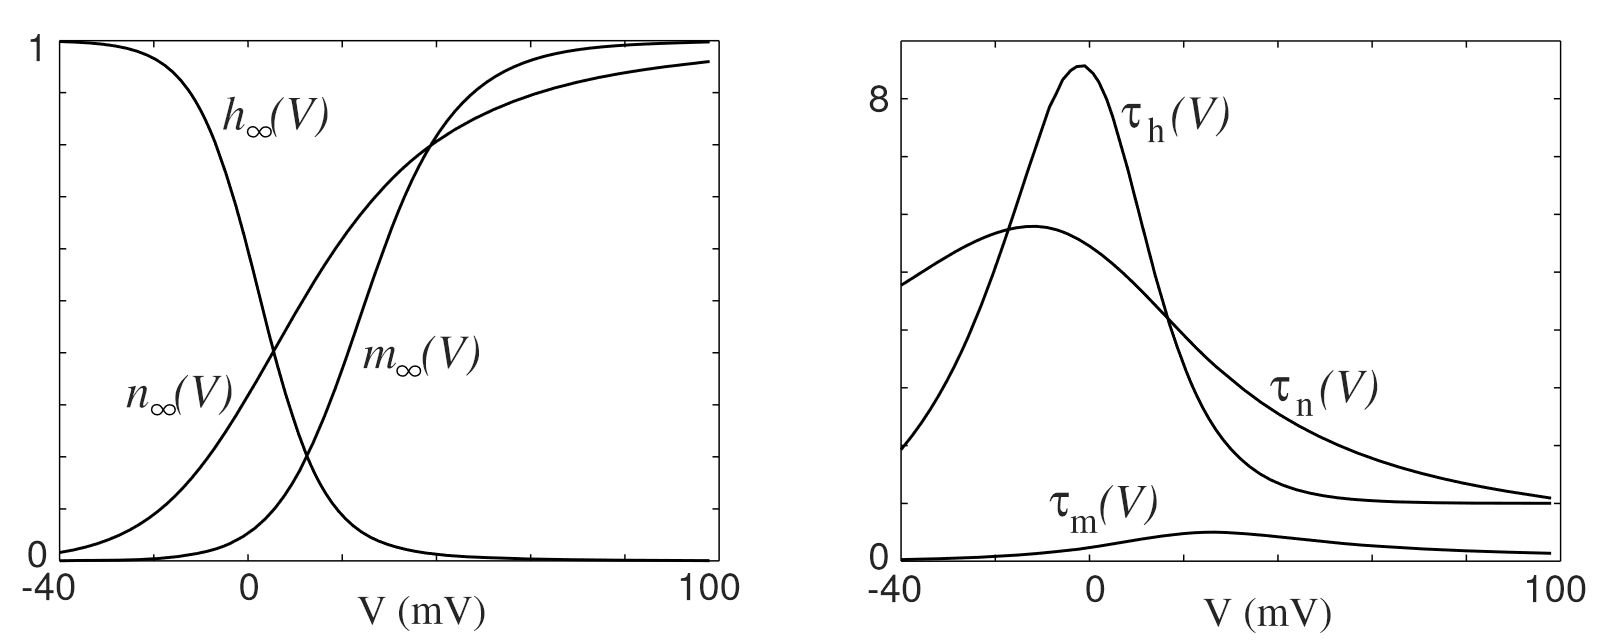
\includegraphics[height=50mm]{chapter1/figures/Hodgkin_Huxley_gates.png}
%     \caption{Steady-state activation and inactivation ($h$) functions 
%     (left) and voltage-dependent time constants (right) in the Hodgking-Huxley model. 
%     This figure is original from \citep{izhikevich_dynamical_2007}. 
%     \textcolor{blue}{(Hacer la propia)}.}
%     \label{fig:hodgkin-huxley-steady-state}
%     \end{center}
% \end{figure}
The squid giant axon membrane primarily features two main currents: transient Na$^{+}$ and persistent K$^{+}$.
Unlike this simplified scenario, most neurons in the central nervous system have additional currents, such as calcium Ca$^{2+}$ current \citep{loewenstein2003temporal}, inward rectifier potassium K$^{+}$ (Kir) current \citep{doi:10.1152/physrev.00021.2009}, hyperpolarization-activated cyclic nucleotide-gated (HCN) current \citep{sartiani2017hyperpolarization}, etc., each displaying diverse activation and inactivation dynamics.
The Hodgkin-Huxley formalism \eqref{eq:gate_dynamics}-\eqref{eq:gate_eqs2} is a widely accepted model to describe their kinetics.
\subsubsection{Wang-Buzsaki model}
The computational model devised by Xiao-Jing Wang and György Buzsáki in 1996 \citep{Wang1996} focuses on elucidating the mechanisms behind the emergence of gamma oscillations in the hippocampus, occurring in a frequency range of approximately 20-100 Hz.
%\footnote{This frequency interval is chosen for historical reasons, as specified in their publication.
%The gamma oscillation frequency range may vary across sources, but a consensus divides it into three subintervals: low, medium, and high gamma. Subsequent chapters will delve into a more detailed discussion of these rhythms.}.
Their research \citep{Wang1996} delved into a computational exploration of rhythmic activity within a network of interconnected inhibitory (GABAergic) fast-spiking neurons. %in different brain regions, such as the neocortex and the hippocampus.
The model, which is based on a modification of the Hodgkin and Huxley model, is tuned to exhibit two salient properties observed in hippocampal and neocortical fast-spiking interneurons.
First, the action potential is followed by a brief afterhyperpolarization (AHP).
Second, the inactivation of the $h$ gate and the activation of the $n$ gate are faster than the activation of the $m$ gate, and the potassium current threshold is higher.
This configuration results in repetitive spikes at high frequencies in response to a constant injected current.
In contrast to \eqref{eq:hodkin_huxley_eqs}, the dynamics of the $m$, $n$, and $h$ gates are described as follows:
\begin{equation}
    \begin{aligned}
            \displaystyle\frac{dm}{dt} & \sim 0 \rightarrow m = m_{\infty},\\
            \displaystyle\frac{dn}{dt} &= \phi(\alpha_n(v)(1-n)-\beta_n(v)),\\
            \displaystyle\frac{dh}{dt} &= \phi(\alpha_h(v)(1-h)-\beta_h(v)),
        \end{aligned}
        \label{eq:wang-buzsaki}
\end{equation}
where
\begin{equation}
    \begin{split}
        \alpha_m(v) & = \displaystyle\frac{0.1(v+35)}{\exp(-0.1(v+35))-1},\\
        \alpha_n(v) & = \displaystyle\frac{-0.01(v+34)}{\exp(-0.1(v+34))-1},\\
        \alpha_h(v) & = 0.07\exp\bigg(-\frac{V+58}{20}\bigg), \\
    \end{split}\quad
    \begin{split}
        \beta_m(v) & = 4\exp\bigg(-\frac{v+60}{80}\bigg), \\
        \beta_n(v)  & = 0.125\exp\bigg(-\frac{v+44}{80}\bigg),\\
        \beta_h(v) & = \displaystyle\frac{1}{\exp(-0.1(v+28))+1}, \\
    \end{split}
\end{equation}
with $g_\text{L}$ = 0.1  mS/cm$^2$, $g_\text{Na}$ = 35 mS/cm$^2$, $g_\text{K}$ = 9 mS/cm$^2$, $E_\text{L}$ = -65  mS/cm$^2$, $E_\text{Na}$ = 55 mS/cm$^2$, $E_\text{K}$ = -90 mS/cm$^2$.
\subsubsection{Izhikevich model}
The Izhikevich model is a simple, yet powerful, spiking neuron model that was proposed by Eugene Izhikevich in 2003 \citep{izhikevich_simple_2003}. 
The model is a two-dimensional system of nonlinear differential equations that captures the essential properties of different types of spiking neurons. 
Previous models of spiking neurons were either too simplistic to capture the complex behavior of real neurons (such as the IAF models) or too complex to allow for analytical and even computational tractability (such as Hodgkin-Huxley model). 
Eugene Izhikevich set out to create a model that was both biologically realistic and mathematically tractable.
It was derived through dimensionality reduction of the Hodgkin-Huxley model, employing methodologies drawn from bifurcation theory \citep{izhikevich_dynamical_2007}.
% To develope his model, Izhikevich used a combination of experimental data and mathematical analysis to identify the key features of different types of spiking neurons. 
% The model could reproduce these features in a simple and computationally efficient way.
The model consists of two variables: a membrane potential $v(t)$ and a recovery variable $u(t)$, which accounts for the activation of K$^{+}$ ionic currents and inactivation of Na$^{+}$ ionic currents, and it provides negative feedback to the membrane potential.
\begin{figure}[!htb]
    \begin{center}
    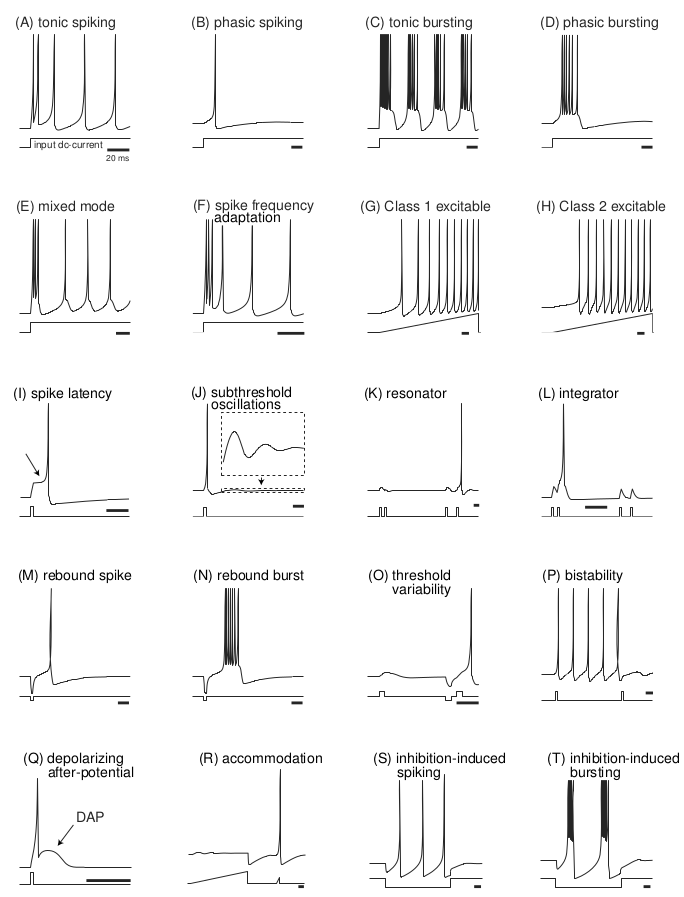
\includegraphics[width=\textwidth]{chapter1/figures/Izhikevich_neuron_patterns.png}
    \caption{\textbf{Different spiking patterns generated by the Izhikevich model}.
    Original figure from \citep{izhikevich_dynamical_2007}.}
    \label{fig:neuron-dynamic-patterns}
    \end{center}
\end{figure}
Similar to integrate-and-fire models, this model also incorporates a reset term. 
After the neuron undergoes a spike and the membrane potential reaches a specified maximum value, $v$ and $u$ undergo a reset. 
The initial form of the model was:
% Initially, the model was presented withdimensionless parameters but with the membrane potential in $mv$ units. but however the part av2 + bv − u  was chosen so that v has mVof differential equations as follows:
\begin{equation}
    \begin{aligned}
        \displaystyle\frac{dv}{dt} &= 0.04v^2+5v+140 -u+ I,\\
        \displaystyle\frac{du}{dt} &= a(bv-u), \\
         t' &: v(t') > 30 mV \rightarrow 
         \begin{cases}
            v(t') &\leftarrow c\\
            u(t') &\leftarrow u(t') + d\\
        \end{cases},
    \end{aligned}
    \label{eq:izhikevich_adimensional}
\end{equation}
where, $v$ and $u$ are dimensionless variables, and $a$,$b$,$c$ and $d$ are dimensionless parameters: $a$ describes the time scale of the recovery variable $u$, $b$ describes the sensitivity of $u$ to the subthreshold fluctuations of the membrane potential $v$, $c$ is the after-spike reset value of the membrane potential, and $d$ is the after-spike reset of $u$ caused by slow-threshold Na$^{+}$ and K$^+$ conductances.
Although the variables are dimensionless, the part $0.04v^2+5v+140$ was obtained by fitting the spike initiation dynamics of a cortical neuron so that the
membrane potential $v$ has mV units and the time t has ms units \citep{izhikevich_simple_2003}.
Later, a dimensional form of his model was published in his famous book \citep{izhikevich_dynamical_2007}:
\begin{equation}
    \begin{aligned}
        C\displaystyle\frac{dv}{dt} &= k(v-v_r)(v-v_t) -u + I, \\
        \displaystyle\frac{du}{dt} &= a\big( b(v-v_r)- u\big), \\
        t' &: v(t') > v_{th} \rightarrow
        \begin{cases}
            v(t') &\leftarrow c\\
            u(t') & \leftarrow u(t') + d\\
        \end{cases},
    \end{aligned}
    \label{eq:izhikevich_dimensional}
\end{equation}
where, $C$ represents the membrane capacitance, $v_r$ denotes the resting membrane potential, and $v_t$ is the instantaneous threshold potential.
While one may perceive this version as having ten free parameters, it can be demonstrated that only four are independent.
Thus, equations \eqref{eq:izhikevich_dimensional} and \eqref{eq:izhikevich_adimensional} are equivalent.
\clearpage
A crucial innovation of the Izhikevich model lies in its ability to capture a wide spectrum of spiking behaviors using just four parameters, as illustrated in Figure \ref{fig:neuron-dynamic-patterns}.
% Moreover, in contrast to more complex models requiring computationally expensive simulations, the Izhikevich model can be analytically solved using straightforward numerical methods, facilitating fast and efficient simulations of large neural networks.
In addition to its computational efficiency, the model provides a favorable balance between simplicity and realism.
In Figure \ref{fig:neuron-model-comparison} a comparison among the most popular neural models is presented, highlighting the optimal equilibrium of the Izhikevich model between efficiency and biological plausibility \citep{izhikevich_dynamical_2007}.
% Given its simplicity and versatility, it has become a popular tool for studying neural dynamics and designing neural networks.

\begin{figure}[!htb]
    \begin{center}
    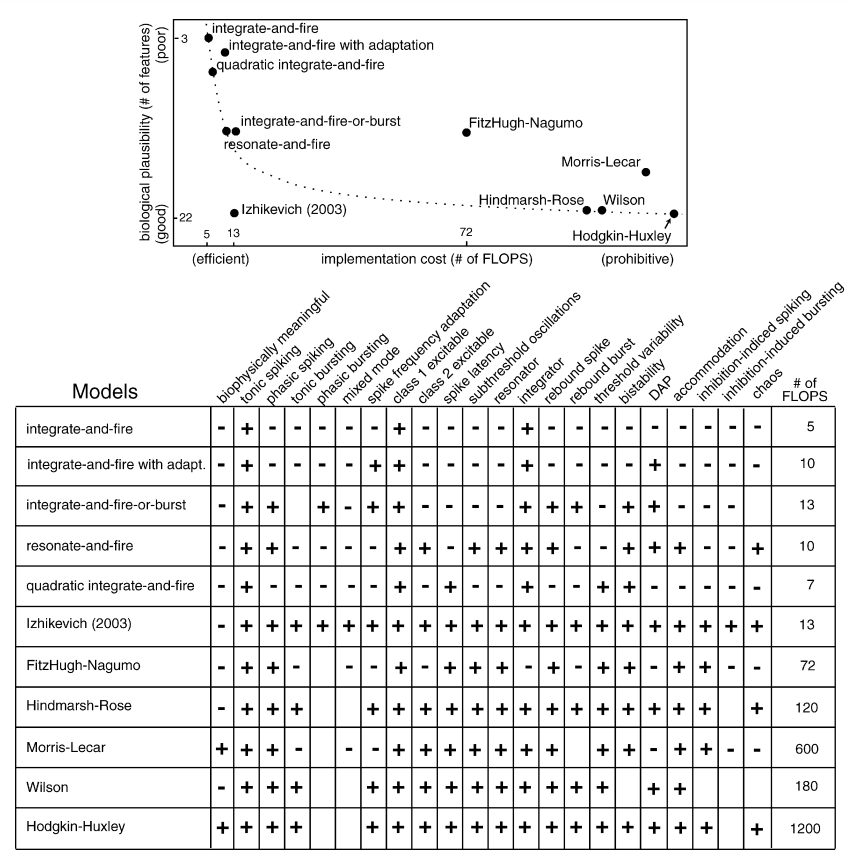
\includegraphics[width=\textwidth]{chapter1/figures/Izhikevich_model_comparison.png}
    \caption{\textbf{Comparison of the most important neuron models}.
    The figure shows the balance between biological plausibility and computational costs.
    The term  "\# of Flops" refers to the total number of operations required for the simulation of the specific model during 1 ms.
    The table shows and compares the properties of all models.
    Original figure from \citep{izhikevich_dynamical_2007}.}
    \label{fig:neuron-model-comparison}
    \end{center}
\end{figure}
\subsubsection{Multicompartimental models}
The neural models presented so far characterize the subthreshold dynamics and, in some cases, the spike generation of the membrane potential, neglecting the neuron structure.
Although suitable for specific modeling goals, this simplification might limit a comprehensive understanding of neural behavior.
The introduction of multicompartmental models addresses this limitation by providing a more detailed and biologically faithful representation of individual neurons.
In these models, neurons are divided into distinct cylindrical compartments (representing dendrites, soma, and axon) with unique electrical properties.

A groundbreaking contribution to the understanding of neuron behavior is the \textbf{Cable Theory}, formulated by Wilfrid Rall in the 1950s–1960s \citep{rall1959branching,rall1962electrophysiology}.
This theoretical framework provides a quantitative analysis of how dendrites and dendritic spines impact synaptic integration.
The core of this theory is the conceptualization of dendrites as conductive cables.
%separated from the extracellular space.
Cables are characterized by an intracellular resistivity $R_i$, a membrane resistivity $R_m$, and a membrane capacitance $C_m$.
If the membrane potential changes at the sealed end of an infinitely extending cable, the voltage will exponentially decay with the distance, as described by the equation: 
\begin{equation}
    \Delta v(x) = \Delta v_0 e^{-\frac{x}{\lambda}},
    \label{eq:cable-equation-decay}
\end{equation}
where $\Delta v_0$ is the voltage change imposed at the end, $\Delta v(x)$ is the voltage change at distance $x$ along the cable, and $\lambda$ is the space constant of the cable given by $\lambda = \sqrt{(d/4)(R_m/R_i)}$, where $d$ is the diameter of the cable.
For transient voltage changes, the decay of the voltage over time is governed by the membrane time constant $\tau = R_mC_m$.
The neural cable equation is given by:
\begin{equation}
    \displaystyle\frac{\partial v}{\partial T} = \displaystyle\frac{\partial^2 v}{\partial X} - v,
\end{equation}
which describes the change of the voltage along the cable in both time and space.
$X$ and $T$ are dimensionless variables given by $X = x/\lambda$ and $T = t/\tau$.
% The cable equation  had initially been applied to axons, but Rall extended its application to dendrites, allowing for the analysis of branching cables and arbitrary dendritic geometries.
\begin{figure}[!htb]%[t]
    \centering
    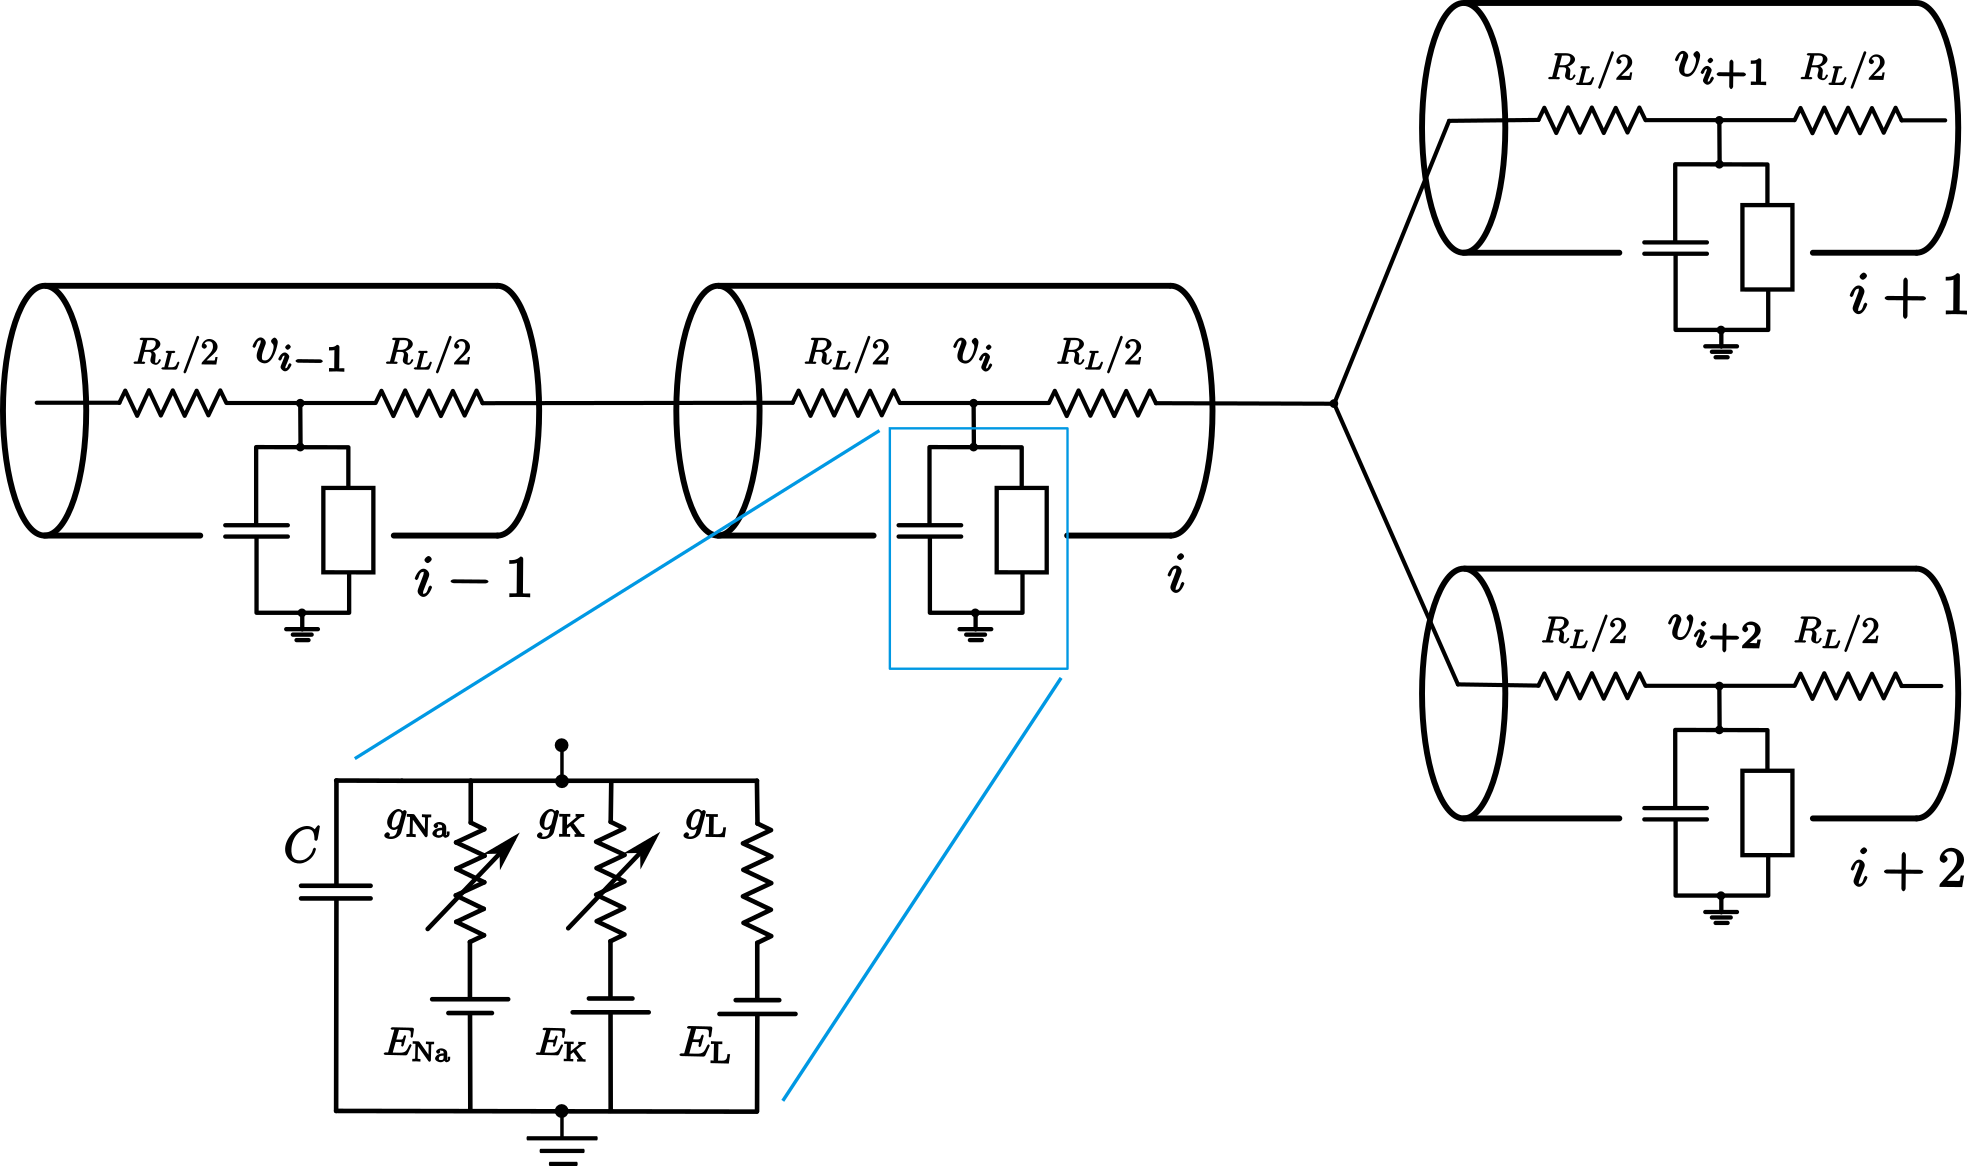
\includegraphics[width=0.9\textwidth]{chapter1/figures/cable_theory.png}
    \caption{\textbf{Multicompartmental modelling}.
    Each cylinder represents a compartment of the neuron and is coupling to its adjacent compartments . 
    In this representation, each the dynamics of each compartment is described by the Hodgkin and Huxley model.}
    \label{fig:cable-theory}
\end{figure}

While the analytical form of the cable equation is suited for passive dendrites with current sources, Rall also considered non-passive properties in dendritic function. 
To address this, he utilized numerical simulations by subdividing the dendritic segments into isopotential compartments and computing membrane potential changes through discrete time steps.
His calculations and simulations yielded numerous insights, highlighting principles such as distance-dependent filtering of synaptic potentials along dendrites and distinct responses to synapses activated in different spatiotemporal patterns.
% Early models, pioneered by Wilfrid Rall and colleagues, used the Cable theory to delve into the impact of dendrites on neuronal computations.
% They predicted sublinear integration due to passive membrane properties, and it was subsequent observed observations in pyramidal neurons of hippocampal region CA1 and in dendritic branches of cereberall neurons.
% Dendrites, with their morphological complexity and diverse ion channels, exhibit non-linear synaptic integration, enabling localized regenerative events like dendritic spikes and spatially restricted plasticity.
% This complexity allows dendrites to function as coincidence and temporal sequence detectors, akin to artificial neural networks \citep{poirazi_illuminating_2020}.

Contemporary multicompartmental models vary significantly, both in their level of biological realism and in their computational complexity \citep{poirazi_arithmetic_2003,cutsuridis_computational_2015,chavlis_dendrites_2017,tzilivaki_hippocampal_2023}.
There is no single answer to the quest of finding the best model as this depends heavily on the question or questions asked.
The only universally applicable advice is rooted in Occam’s razor: the optimal model is one that is sufficiently detailed to integrate, gate, and/or amplify resulting depolarizations, modulate signal propagation, and underlie the induction of dendritic spikes \citep{poirazi_illuminating_2020}.
Figure \ref{fig:cable-theory} illustrates a circuit schematics of a piece of a generic neuron model, where coupled compartments have their own dynamics.

\subsection{Classification of neural models}
Neurons exhibit diverse firing patterns and an essential measure for understanding their behavior is the \textbf{phase response curve} (PRC), which characterizes how spike timing changes in response to external stimuli \citep{hansel1995synchrony}.
PRCs are broadly categorized into \textbf{Type I} and \textbf{Type II} excitability.
\textbf{Type I} neurons primarily show phase advances in response to excitatory stimuli, while \textbf{Type II} neurons exhibit both advance and delay responses.
This classification extends to a neuron's frequency-current $f-I$ relation, where \textbf{Type I} neurons have arbitrarily low frequencies at firing thresholds, and \textbf{Type II} neurons display a finite, non-zero firing frequency at threshold \citep{ermentrout2001effects,schultheiss2011phase,fink_cellularly-driven_2011}.
\textbf{Type I} neurons exhibit  gradual transition from quiescence to repetitive spiking and act as integrators, \textbf{Type II }neurons show, in contrast, an abrupt transition and act as resonators \citep{izhikevich_dynamical_2007} (see top panels in Figure \ref{fig:PRC}).

It is important to emphasize that this classification is a simplification, and in reality, neuronal behavior exists along a continuum. Moreover, the classification may depend on the specific firing properties under consideration, with some neurons showcasing mixed characteristics or transitioning between types under different conditions.
\begin{figure}[!htb]
    \centering
    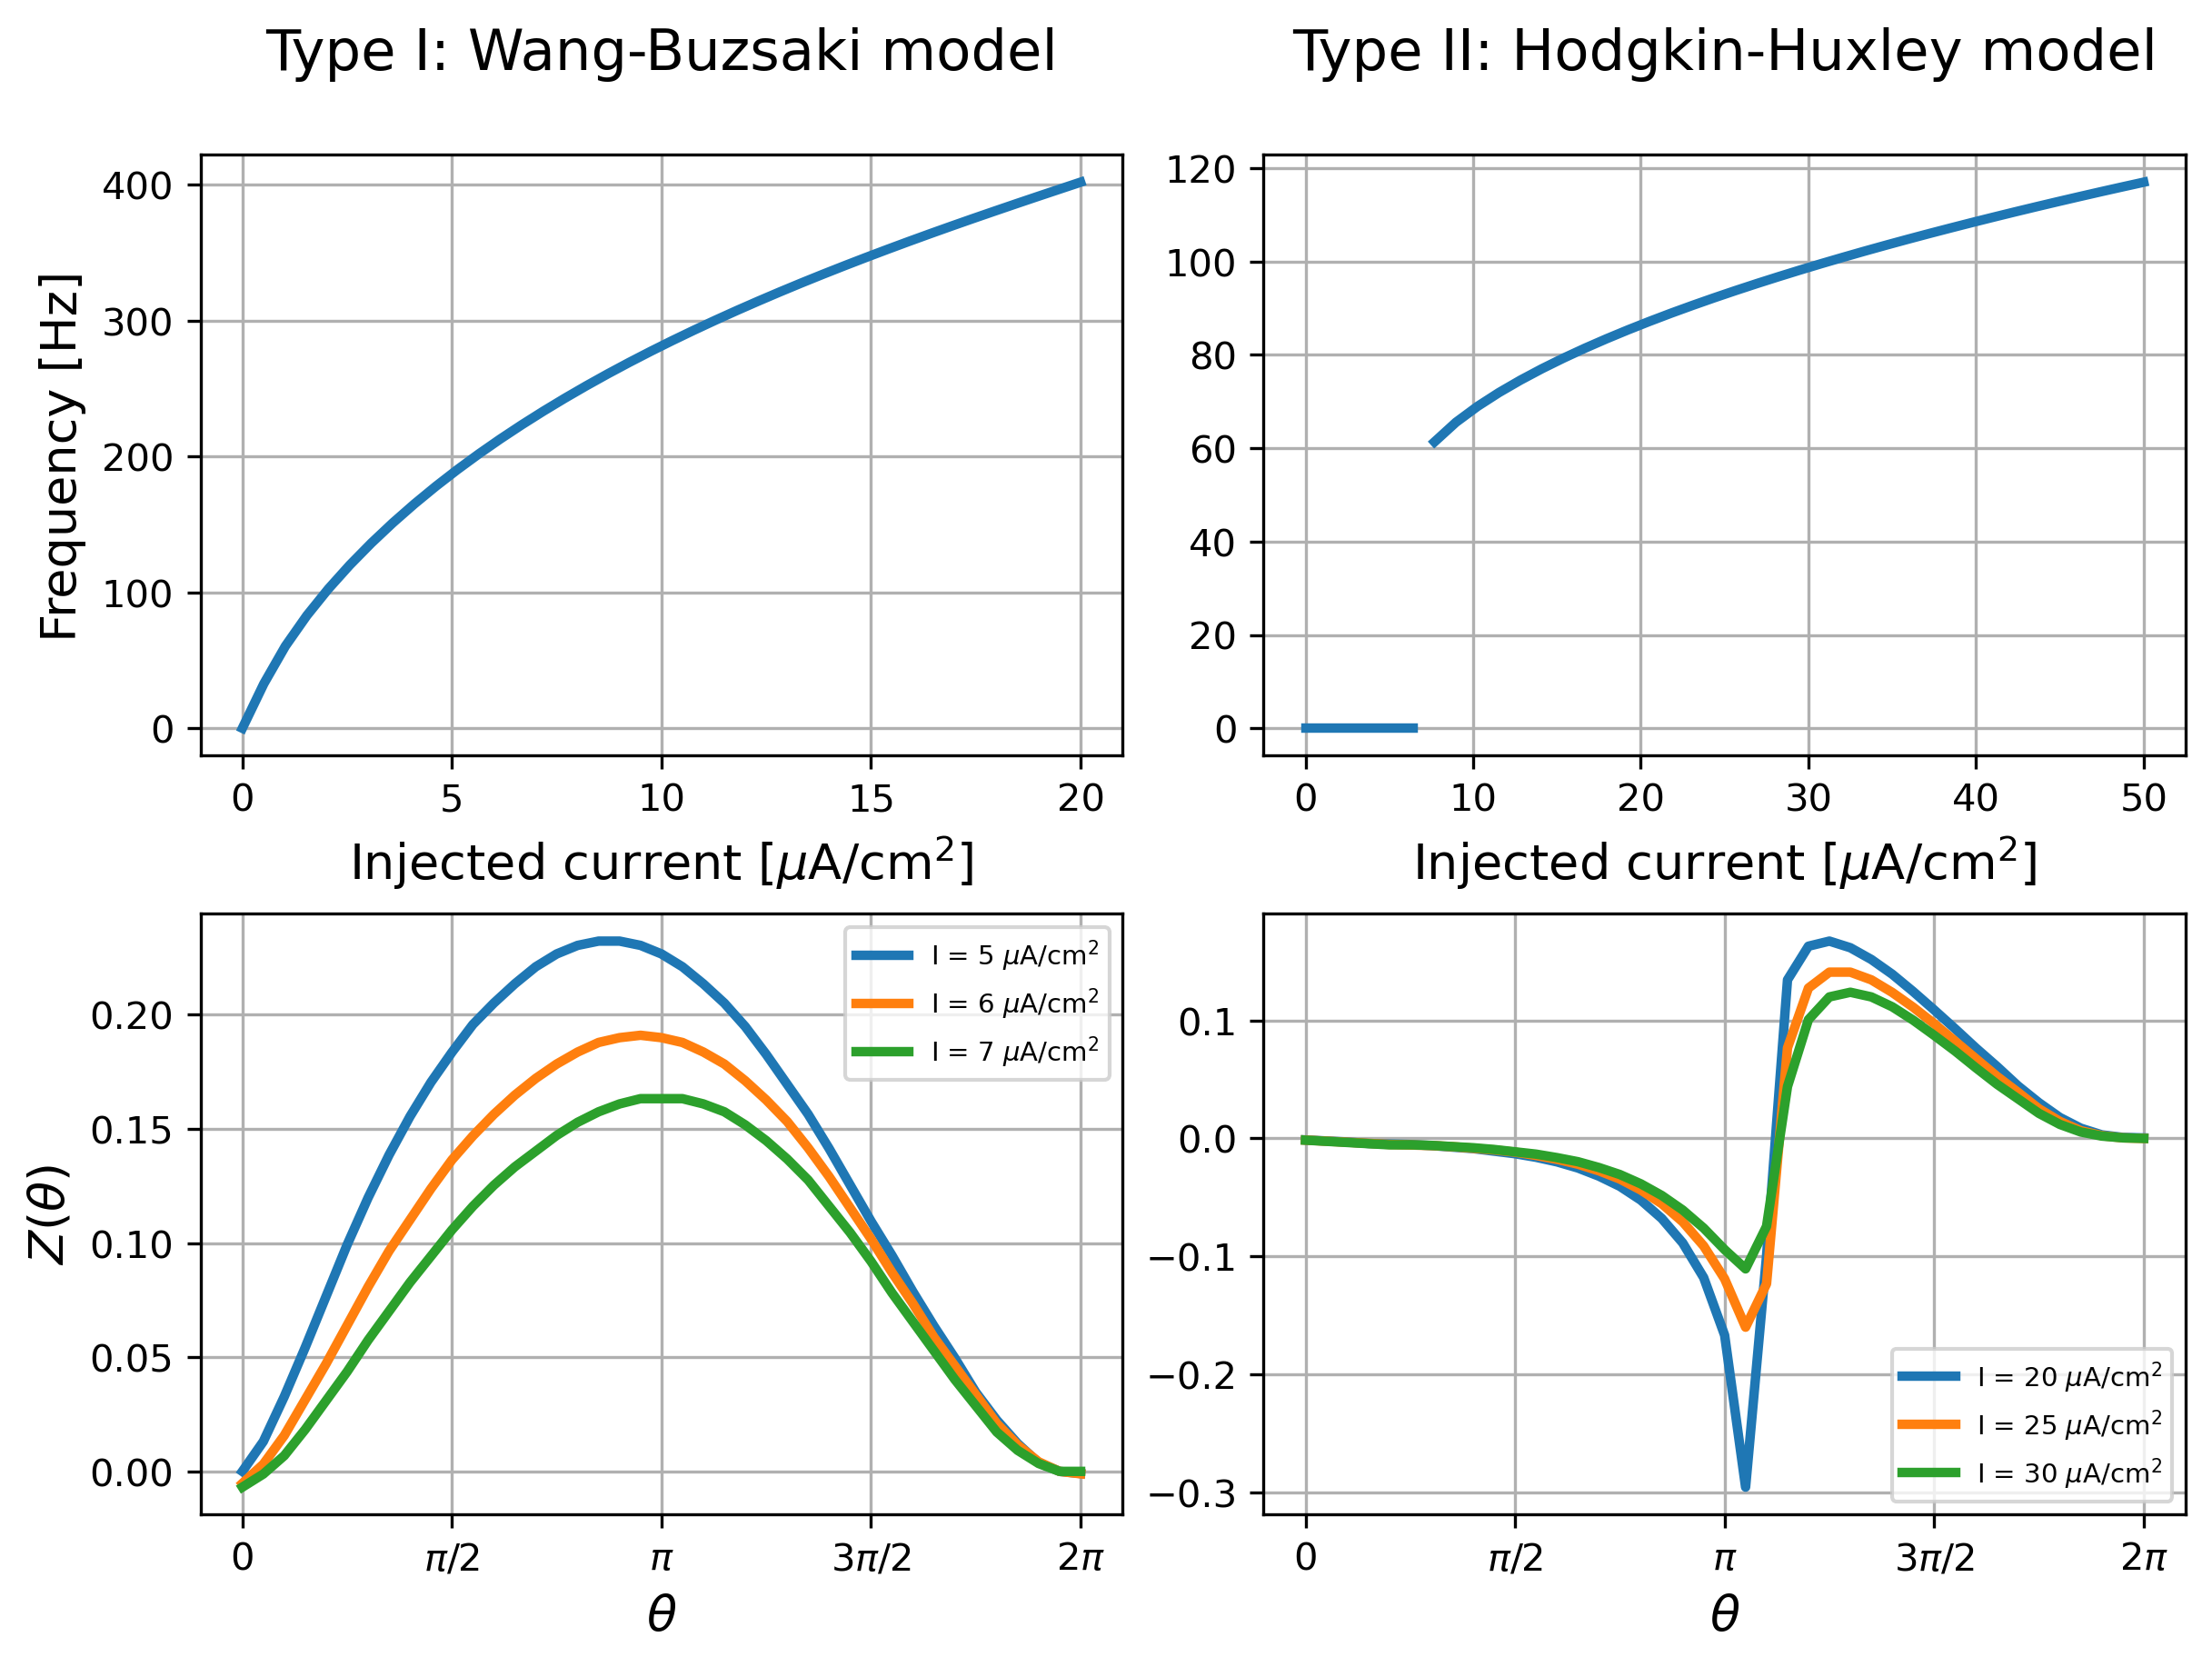
\includegraphics[width=\textwidth]{chapter1/figures/PRCs.png}
    \caption{\textbf{Type I and Type II neurons}.
    The Wang-Buszaki and the Hodgking-Huxley model, respectively.
    Comparative between the $f-I$ curves and the PRCs.
    PRCs were computed by using a current step of $2$ ms with an amplitude of 10 $\mu$A/cm$^2$.}
    \label{fig:PRC}
\end{figure}
\subsubsection{Phase Response Curve}
The \textbf{phase response curve} $Z(\theta)$ elucidates how the timing or the phase of a neuron firing is affected by brief perturbations applied during the ongoing regular firing cycle.
This regular firing can be considered as a stable oscillator with a period $T$, or angular frequency $\omega = 2\pi/T$.
In this case, its state is described only with its phase $\theta$, and being $d\theta/dt = \omega$.
In the absence of any external perturbation, the neuron spikes at $\theta = kT$, where $k$ is a positive integer.
If the neuron receives a short perturbation with a small amplitude $\Pi(\theta)$, the impact of this perturbation on the next spike is described by \citep{izhikevich_dynamical_2007}:
\begin{equation}
\begin{aligned}
    \displaystyle\frac{d\theta}{dt} &= \omega + \Pi(\theta)Z(\theta),\\
    Z(\theta) &= (T-T'(\theta))\displaystyle\frac{2\pi}{T}, 
    \label{eq:PRC}
\end{aligned}
\end{equation}
where $T'(\theta)$ represents the interspike interval between the previous and next spike after the perturbation.
While \textbf{type I} neurons exhibit a purely positive PRC, indicating an advancement of the next spike.
In contrast, \textbf{type II} neurons exhibit a biphasic behavior, advancing or delaying the next spike based on the phase of the cycle at which the perturbation is applied.
%PRCs reveal information about the synchronization properties of the neurons \citep{izhikevich_simple_2003, torben-nielsen_comparison_2010.
Figure \ref{fig:PRC} illustrates the PRCs and the $f-I$ curves of the Wang-Buzsaki and Hodgkin-Huxley models, serving as examples of type I and type II neurons, respectively.

\end{document}
things written before and discarded.
\textbf{Current-frequency curves} depict the relationship between the injected current and the resulting firing rate of a neuron. In Type I neurons, the current-frequency curve typically exhibits a linear or near-linear relationship. As the injected current increases, the firing rate of the neuron also increases in a graded manner. In contrast, Type II neurons display a nonlinear current-frequency relationship. Initially, as the injected current increases, the firing rate rises steeply, indicating a rapid onset of firing. However, as the current continues to increase, the firing rate saturates or even decreases due to the presence of adaptation mechanisms.

On the ohter hand, \textbf{Phase response curves} describe how the timing or phase of a neuron's firing is influenced by brief perturbations applied during the ongoing regular firing cycle.
This regular firing can be seen as stable oscillator with period $T$ (or angular frequency $\omega = 2\pi/T$) and only the phase $\theta$ to describe its state ($d\theta/dt = \omega$). 
In the abscence of any external input the neuron spikes at $\theta = kT$, where $k$ is a positive integer. 
Now, if the neuron receives a short input with small amplitude $\Pi(\theta)$, then the influence of this perturbation on the next spike is descirbed by:

The current-frequency curves and phase response curves provide complementary information about the firing properties of neurons. Type I neurons exhibit a linear current-frequency relationship and a monotonic PRC, indicating continuous firing behavior with consistent response properties. Type II neurons, on the other hand, show a nonlinear current-frequency relationship and a non-monotonic PRC, indicating adaptive firing behavior and sensitivity to input timing.

Based on the firing pattern, neural models can be classified as \textbf{Type I} and \textbf{Type II}:
\begin{enumerate}
    \item \textbf{Type I} neurons are characterized by continuous firing patterns. When these neurons receive a constant input, they exhibit a steady firing rate. 
    This firing rate remains relatively constant as long as the input remains within a certain range.
    \item \textbf{Type II} neurons exhibit a more complex firing pattern compared to Type I neurons. These neurons display a rapid onset of firing followed by adaptation, where the firing rate decreases over time in response to a constant input. This adaptation behavior allows Type II neurons to selectively respond to changes in the input rather than steady stimuli.
\end{enumerate}
It is important to remark that the Type I and Type II classification is a simplification, and in reality, neuronal behavior can vary along a continuum. Additionally, the classification can depend on the specific firing properties being considered, and some neurons may exhibit mixed characteristics or transition between types under different conditions.

The classification of neural models into \textbf{Type I} and \textbf{Type II} classes can also be related to the \textbf{current-frequency curves} and the \textbf{phase response curves} (PRC)\citep{izhikevich_dynamical_2007}. These curves provide insights into the firing properties and dynamics of neuron.

% \begin{figure}
%     \centering
%     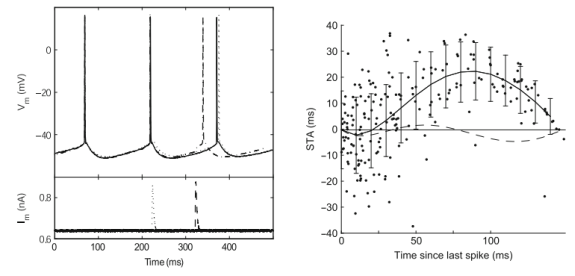
\includegraphics[width=120mm]{chapter1/figures/PRC_experimental.png}
%     \caption{Experimental PRC...(\textbf{cita})}
%     \label{fig:PRC-experimental}
% \end{figure}
